%%%%%%%%%%%%%%%%%%%%%%%%%%%%%%%%%%%%%%%%%
% Short Sectioned Assignment
% LaTeX Template
% Version 1.0 (5/5/12)
%
% This template has been downloaded from:
% http://www.LaTeXTemplates.com
%
% Original author:
% Frits Wenneker (http://www.howtotex.com)
%
% License:
% CC BY-NC-SA 3.0 (http://creativecommons.org/licenses/by-nc-sa/3.0/)
%
%%%%%%%%%%%%%%%%%%%%%%%%%%%%%%%%%%%%%%%%%

%----------------------------------------------------------------------------------------
%	PACKAGES AND OTHER DOCUMENT CONFIGURATIONS
%----------------------------------------------------------------------------------------

\documentclass[paper=a4, fontsize=11pt]{scrartcl} % A4 paper and 11pt font size
\usepackage{amsmath,amsfonts,graphicx}

\usepackage{booktabs}
%\usepackage{algpseudocode}
\usepackage{algorithm}
\usepackage{algorithmicx}
\usepackage{algpseudocode}
\usepackage[top=2cm, bottom=2cm, left=2cm, right=2cm]{geometry}

\usepackage{listings}
\usepackage{color}
\usepackage{xcolor}
\definecolor{dkgreen}{rgb}{0,0.6,0}
\definecolor{gray}{rgb}{0.5,0.5,0.5}
\definecolor{mauve}{rgb}{0.58,0,0.82}
\lstset{frame=tb,
     %language=Java,
     aboveskip=3mm,
     belowskip=3mm,
     showstringspaces=false,
     columns=flexible,
     basicstyle = \ttfamily\small,
     numbers=none,
     numberstyle=\tiny\color{gray},
     keywordstyle=\color{blue},
     commentstyle=\color{dkgreen},
     stringstyle=\color{mauve},
     breaklines=true,
     breakatwhitespace=true,
     tabsize=3
}

%\usepackage[]{algorithm2e}

\usepackage[T1]{fontenc} % Use 8-bit encoding that has 256 glyphs
\usepackage{fourier} % Use the Adobe Utopia font for the document - comment this line to return to the LaTeX default
\usepackage[english]{babel} % English language/hyphenation
\usepackage{amsmath,amsfonts,amsthm} % Math packages

\usepackage{lipsum} % Used for inserting dummy 'Lorem ipsum' text into the template

\usepackage{sectsty} % Allows customizing section commands
\allsectionsfont{\centering \normalfont\scshape} % Make all sections centered, the default font and small caps

\usepackage{fancyhdr} % Custom headers and footers
\pagestyle{fancyplain} % Makes all pages in the document conform to the custom headers and footers
\fancyhead{} % No page header - if you want one, create it in the same way as the footers below
\fancyfoot[L]{} % Empty left footer
\fancyfoot[C]{} % Empty center footer
\fancyfoot[R]{\thepage} % Page numbering for right footer
\renewcommand{\headrulewidth}{0pt} % Remove header underlines
\renewcommand{\footrulewidth}{0pt} % Remove footer underlines
\setlength{\headheight}{13.6pt} % Customize the height of the header

\numberwithin{equation}{section} % Number equations within sections (i.e. 1.1, 1.2, 2.1, 2.2 instead of 1, 2, 3, 4)
\numberwithin{figure}{section} % Number figures within sections (i.e. 1.1, 1.2, 2.1, 2.2 instead of 1, 2, 3, 4)
\numberwithin{table}{section} % Number tables within sections (i.e. 1.1, 1.2, 2.1, 2.2 instead of 1, 2, 3, 4)

\setlength\parindent{0pt} % Removes all indentation from paragraphs - comment this line for an assignment with lots of text

%----------------------------------------------------------------------------------------
%	TITLE SECTION
%----------------------------------------------------------------------------------------

\newcommand{\horrule}[1]{\rule{\linewidth}{#1}} % Create horizontal rule command with 1 argument of height

\title{	
\normalfont \normalsize 
\textsc{The University of Melbourne } \\ [25pt] % Your university, school and/or department name(s)
\horrule{0.5pt} \\[0.4cm] % Thin top horizontal rule
\huge COMP90038 Algorithms and Complexity SM2, 2018
Assignment 1 \\ % The assignment title
\horrule{2pt} \\[0.5cm] % Thick bottom horizontal rule
}

\author{Peiyong Wang $\,$ 955986} % Your name

\date{\normalsize\today} % Today's date or a custom date

\begin{document}

\maketitle % Print the title



\section{Problem One}
\paragraph{a} Clearly this algorithm searches in an array for a value which equals to its index, like A[9]=9.
\paragraph{b} The algorithm firstly examines whether A[lo] > lo or A[hi] < hi. If so, it means all values are bigger or smaller than their indexes, and in this situation the algorithm will return -1, indicating there is no possibility in the input array that $\exists i \in  \mathbb{N^+},\, s.t. A[i] = i $. If the input array satisfy this condition, then the algorithm will use hi and lo to compute mid and check whether A[mid] = mid. If so, return mid; if not, the algorithm will split the array into two halves and if A[mid] is bigger than mid the algorithm will continuing its search in the lower half, otherwise it will search in the higher half of the input array and recursively call the function itself.

\vbox{ }

However, to make this algorithm work fine, the input array must only have on value that equals to its key, and there should be no duplicates.
If it has many values that they all equal to their keys repectively, the algorithm will only find one. If the input array have duplicates there is a chance that there will be a A[$lo$]>$lo$ or A[$hi$]<$hi$ 
situation, which won't pass the first if-clause in the algorithm.
\section{Problem Two}


See Algorithm 1.

\begin{algorithm}
        \caption{Count the number of occurrences of a certain integer $x$ in an array $A[]$}
        \begin{algorithmic}[1] %每行显示行号
            \Require  $Array$ $A[\cdot]$,$Length\;of\;the\;array$ n, $Integer$ x
            \Ensure   Number of occurrence of integer x  
            \Function {NumberCount}{$A[\cdot], x,n$}
            
            	\State $firstApperence \gets $\Call{FirstOccurrenceSearch}{$A[\cdot]$,0,$n-1$,$x$,$n$}
            	
            	\If{$firstApperence=-1$}
            	\State \Return $firstApperence$
            	\EndIf
            	
            	\State $lastApperence\gets$ \Call{LastOccurrenceSearch}{$A[],firstApperence,n-1,x,n$}
            	\State \Return $lastApperence-firstApperence+1$
            	
                %\State $result \gets 0$
                
                %\If {$high \geqslant low$}
                    %\State $mid \gets (high + low) // 2$   \#"//" means integer division
                    %\State $result \gets result +$ \Call{MergerSort}{$Array, left, middle$}
                    %\State $result \gets result +$ \Call{MergerSort}{$Array, middle, right$}
                    %\State $result \gets result +$ \Call{Merger}{$Array,left,middle,right$}
                %\EndIf
                %\If {$mid = 0 \, OR x > A[mid-1]$}
                %	\State \Return $mid$
                %\Else 
                %	\If {$x>A[mid]$}
                %		\State \Return 
                
                 %\Return{$result$}
            \EndFunction
           \State
            \Function{FirstOccurrenceSearch}{$A[\cdot],low, high,x,n$}
            
            \If{$high \geqslant low$}
            \State $mid\gets(low + high)//2$ \Comment "//" means integer division
            \EndIf
            \If{$\{mid = 0 \; OR\;  x>A[mid-1]\}\; AND\; \{A[mid]=x\}$} 
            \State \Return $mid$
            \Else
            	\If{$x>A[mid]$}
            	\State \Return \Call{FirstOccurrenceSearch}{$A[\cdot],mid+1,high,x,n$}
            	\Else
            	\State \Return \Call{FirstOccurrenceSearch}{$A[\cdot],low,mid-1,x,n$}
            	\EndIf
            \EndIf
            \State \Return -1
            
            \EndFunction
            
            \State
            \Function{LastOccurrenceSearch}{$A[\cdot],low,high,x,n$}
            
            \If{$high \geqslant low$}
            \State $mid\gets(low + high)//2$ \Comment "//" means integer division
            \EndIf
            \If{$\{mid = n-1 \; OR\;  x<A[mid-1]\}\; AND\; \{A[mid]=x\}$} 
            \State \Return $mid$
            \Else
            	\If{$x<A[mid]$}
            	\State \Return \Call{LastOccurrenceSearch}{$A[\cdot],low, mid-1, x,n$}
            	\Else
            	\State \Return \Call{LastOccurrenceSearch}{$A[\cdot],mid+1, high,x,n$}
            	\EndIf
            \EndIf
            \State \Return -1
            
            

            \EndFunction
            
            %\Function{Merger}{$Array, left, middle, right$}
             %   \State $i\gets left$
              %  \State $j\gets middle$
               % \State $k\gets 0$
               % \State $result \gets 0$
               % \While{$i<middle$ \textbf{and} $j<right$}
                %    \If{$Array[i]<Array[j]$}
                 %       \State $B[k++]\gets Array[i++]$
                  %  \Else
                   %     \State $B[k++] \gets Array[j++]$
                    %    \State $result \gets result + (middle - i)$
                    %\EndIf
                %\EndWhile
                %\While{$i<middle$}
                %    \State $B[k++] \gets Array[i++]$
                %\EndWhile
                %\While{$j<right$}
                %    \State $B[k++] \gets Array[j++]$
                %\EndWhile
                %\For{$i = 0 \to k-1$}
                %    \State $Array[left + i] \gets B[i]$
                %\EndFor
                %\State \Return{$result$}
            %\EndFunction
        \end{algorithmic}
    \end{algorithm}


\section{Problem Three}
\paragraph{a} From Figure 3.1, which is a "state tree" that in this tree a path starts from node "start" (but not include node start) and ends at a node that in the binary tree's bottom indicates a possible collections of booleans that could satisfy the formula. For example, the array $A = [true, false, false]$ in the question can be converted to a path starts from node 1, then go to node 4 and ends at node 10. So we can tell that for the worst case scenario of the algorithm stated in the question, we need to traverse all the paths in the state tree. The time complexity of binary tree traversal is $O(n+n-1)=O(n)$, where $n$ is the number of nodes in the binary tree. If we let $n=number\;of\;elements\;in\;array\;A$, then the total number of nodes in the binary tree is $1 + \sum_{i=0}^n 2\cdot 2^i = 2^{n+2}-1 $. So the worst case time complexity is $O(2^{n+2}-1)=O(2^n)$

\begin{figure}[htbp!]
		\centering
		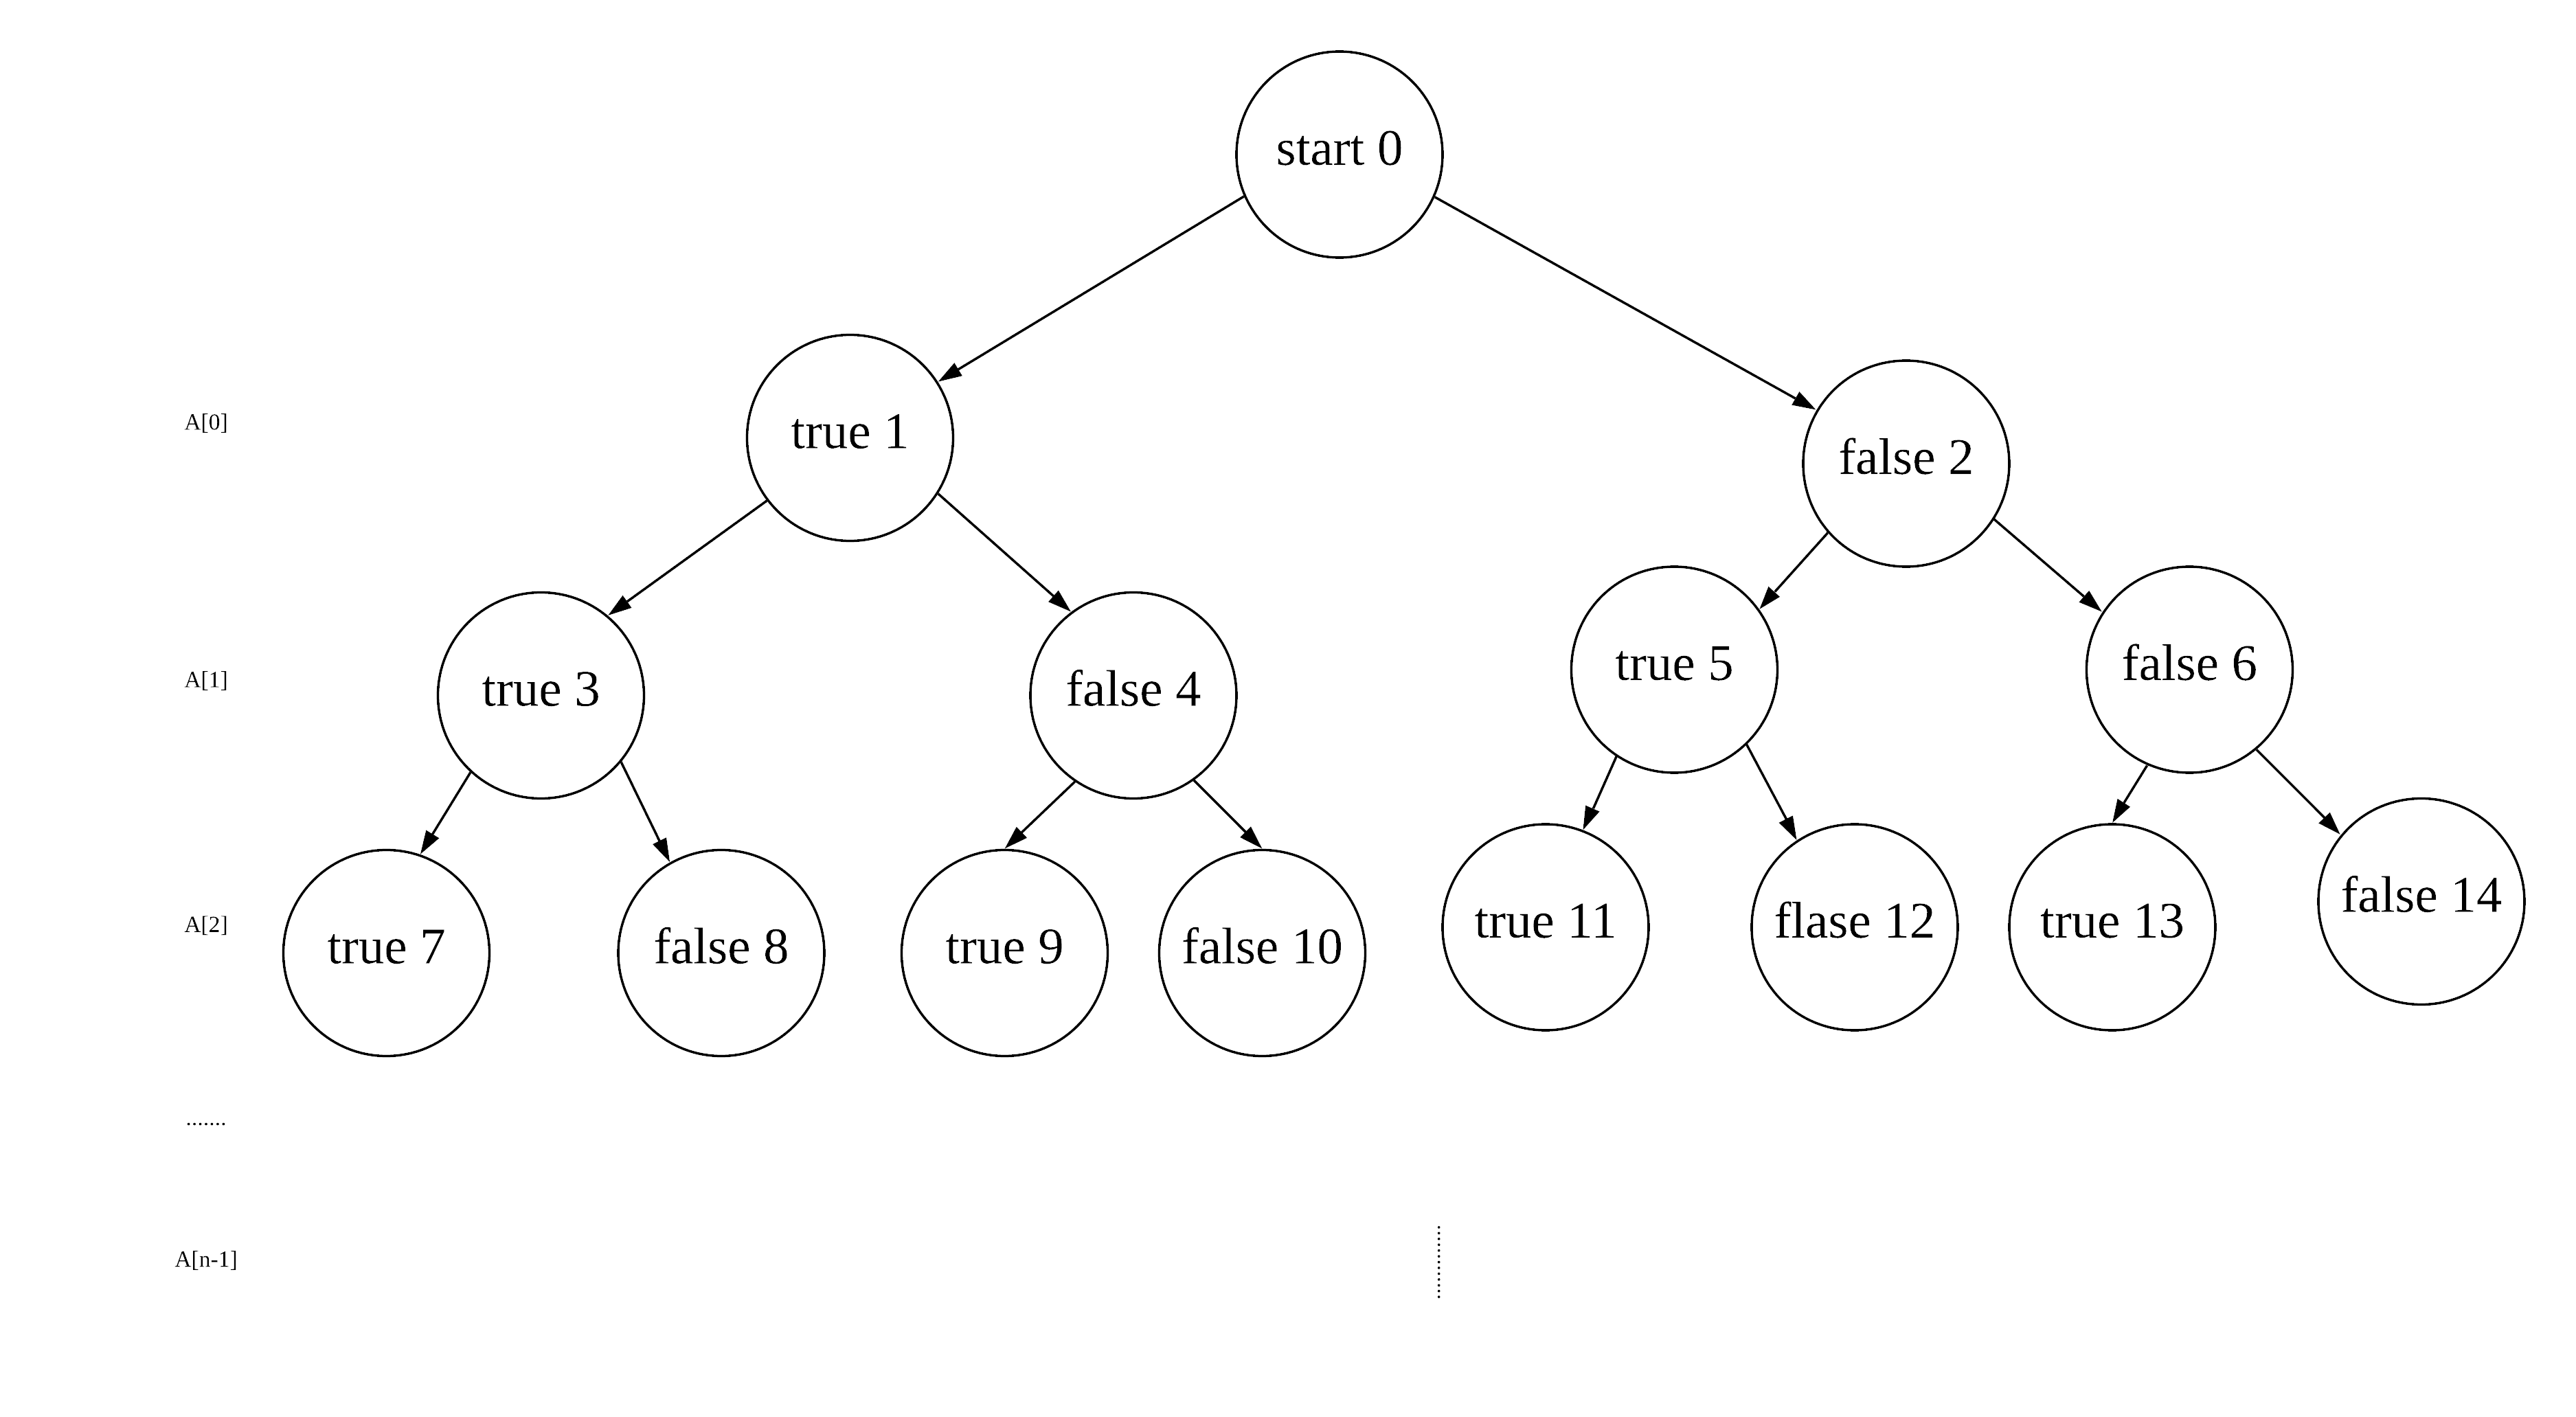
\includegraphics[width=1.0\textwidth]{fig1.png}
		\caption{State Tree}%\label{book}
		\vspace{-1em}
\end{figure}

\paragraph{b} 
From paragraph A, we can easily see that:
\begin{align}
	\begin{split}
		C(1) &= 2
	\end{split}
\end{align}

\begin{align}
	\begin{split}
		C(n) &= 2C(n-1)
	\end{split}
\end{align}

Then we can have that:

\begin{align}
	\begin{split}
		C(n) &= 2C(n-1)\\
		&= 2(2(C(n-2)))\\
		&= \cdots\\
		&= 2^{n-1}C(1)\\
		&= 2^n
	\end{split}
\end{align}

So the time complexity is $\Theta (2^n) $.

\section{Problem Four}

\paragraph{a} 
See Algorithm 2.
\begin{algorithm}
	\caption{Follow a given route linked list to move to the destination and then go back.}
	\begin{algorithmic}[1]
		\Require head of the linked list of route
		\Function{GoAndBack}{$head$}
			\State $p\gets head$  \Comment Starting from the home base
			\State $goBack\gets$ empty stack
			%\State $i\gets 0$
			\While{$p$ is not null}
				\State \Call{Move}{$p$.val}
				\State $goBack$.push($p.val$) \Comment Push the current position to the stack
				\State $p\gets p$.next
				%\State $i\gets i+1$
            \EndWhile
            \State $hashBack\gets$ \{ "N":"S","E":"W","S":"N","W":"E" \}\Comment This is a hash table that stores the opposite directons, like a dictionary in Python, eg: $hashBack$("N")="S".
			\While{$goBack$ is not null}
				\State \Call{Move}{$hashBack$($goBack$.pop)} \Comment Pop the top element of the stack,use the hash table to find its opposite direction, and call the Move function
			\EndWhile
			
		\EndFunction
	\end{algorithmic}

\end{algorithm}

\paragraph{b} See Algorithm 3.
\begin{algorithm}
	\caption{Use BFS to search the shortest route from home base to goal}
	\begin{algorithmic}[1]
		\Require Graph adjacency matrix $A[\cdot,\cdot]$, start, goal
		\Ensure Route list
		\Function{ShortestPath}{$A[\cdot,\cdot],start, goal$}
			\State $pathOfNodes\gets$\Call{BFSPaths}{$start$}
			\State $reverseRoute\gets$ empty list []
			\State $currentVortex\gets goal$
			\While{$pathOfNodes[currentVortex]\neq -1$}
				\State $reverseRoute$.append($currentVortex$)
				\State $currentVortex\gets pathOfNodes[currentVortex]$
			\EndWhile
			\State $routeList\gets $empty list []
			\State $j\gets reverseRoute$.length
			\While{$j\geq 1$}
				$routeList$.append($A[reverseRoute[j],reverseRoute[j-1]]$)
            \EndWhile
            \State $routeLinkedList\gets$ empty linked list with head q and length is the same as $routeList$
            \For{$k = 0; k < routeList.length; k++$}
                \State $q.value\gets routeList[k]$
                \State $q\gets q.next$
            \EndFor
			\State \Return $routeLinkedList$
		\EndFunction
        \State
        
		\Function{BFSPaths}{start}
			\For{each vortex $v$}
				\State $flag[v]\gets false$
				\State $pathList[v]\gets -1$ \Comment Maintain a list that records what is the previous node of a node in the BFS searching path
			\EndFor
			\State $Q\gets empty\; queue$
			\State $flag[start]\gets true$
			\State \Call{Enqueue}{$Q$,$start$}
			\While{$Q$ is not empty}
				\State $v\gets$ \Call{Dequeue}{$Q$}
				\For{each $w$ adjacent to $v$}
					\If{$flag[w]=true$}
						\State $flag[w]\gets true$
						\State $pathList[w]\gets v$
						\State \Call{Enqueue}{$Q, w$}
					\EndIf
				\EndFor
			\EndWhile
			\State \Return $pathList$
		\EndFunction
	\end{algorithmic}		
\end{algorithm}




\end{document}



%\begin{align} 
%\begin{split}
%(x+y)^3 	&= (x+y)^2(x+y)\\
%&=(x^2+2xy+y^2)(x+y)\\
%&=(x^3+2x^2y+xy^2) + (x^2y+2xy^2+y^3)\\
%&=x^3+3x^2y+3xy^2+y^3
%\end{split}					
%\end{align}





%\begin{tabbing}
%\hspace*{.25in} \= \hspace*{.25in} \= \hspace*{.25in} \= \hspace*{.25in} \= \hspace*{.25in} \=\kill
%\>$Euclid(m,n)=$ \\
%\>\> {\bf while} n$ \neq $ 0 \\
%\>\>\> r $ \leftarrow $ $m$ mod $n$  \\
%\>\>\>  m $\leftarrow$n\\
%\>\>{\bf return} m 
%\end{tabbing}

%Python code:
%\begin{lstlisting}[language = python]
%def gcd(m,n):
%	while n != 0:
%		r = m % n
%		m = n
%		n = r
%	return m
%\end{lstlisting}


%\paragraph{Heading on level 4 (paragraph)}




%\begin{tabbing}
%	\hspace*{.25in} \= \hspace*{.25in} \= \hspace*{.25in} \= \hspace*{.25in} \= \hspace*{.25in} \=\kill
%	{\bf function} find (A,x,n)\\
%	\> j $\leftarrow$ 0\\
%	\> {\bf while} j < n\\
%	\>\> {\bf if} A[j]=x\\
%	\>\>\>  {\bf return} j  \\
%	\>\> j $\leftarrow$ j+1\\
%	\> {\bf return} -1
%\end{tabbing}


%\begin{figure}[htbp!]
%		\centering
%		\includegraphics[width=0.6\textwidth]{lec26.png}
%		\caption{Linked List}%\label{book}
%		\vspace{-1em}
%\end{figure}






%\begin{align}
%A = 
%\begin{bmatrix}
%A_{11} & A_{21} \\
%A_{21} & A_{22}
%\end{bmatrix}
%\end{align}



%\begin{algorithm}
 %       \caption{Count the number of occurrences of a certain integer $x$ in an array $A[]$}
  %      \begin{algorithmic}[1] %每行显示行号
   %         \Require  $Array$ A[],$Length\;of\;the\;array$ n, $Integer$ x
    %        \Ensure   Number of occurrence of integer x  
     %       \Function {NumberCount}{$A[], x,n$}
      %      
       %     	\State $firstApperence \gets $\Call{FirstOccurrenceSearch}{$A[]$,0,$n-1$,$x$,$n$}
            	
        %    	\If{$firstApperence=-1$}
         %   	\State \Return $firstApperence$
          %  	\EndIf
            	
           % 	\State $lastApperence\gets$ \Call{LastOccurrenceSearch}{$A[],firstApperence,n-1,x,n$}
            %	\State \Return $lastApperence-firstApperence+1$
            	
                %\State $result \gets 0$
                
                %\If {$high \geqslant low$}
                    %\State $mid \gets (high + low) // 2$   \#"//" means integer division
                    %\State $result \gets result +$ \Call{MergerSort}{$Array, left, middle$}
                    %\State $result \gets result +$ \Call{MergerSort}{$Array, middle, right$}
                    %\State $result \gets result +$ \Call{Merger}{$Array,left,middle,right$}
                %\EndIf
                %\If {$mid = 0 \, OR x > A[mid-1]$}
                %	\State \Return $mid$
                %\Else 
                %	\If {$x>A[mid]$}
                %		\State \Return 
                
                 %\Return{$result$}
            %\EndFunction
           %\State
            %\Function{FirstOccurrenceSearch}{$A[],low, high,x,n$}
            
      %      \If{$high \geqslant low$}
      %      \State $mid\gets(low + high)//2$ \Comment "//" means integer division
      %      \EndIf
      %      \If{$\{mid = 0 \; OR\;  x>A[mid-1]\}\; AND\; \{A[mid]=x\}$} 
      %      \State \Return $mid$
      %      \Else
      %      	\If{$x>A[mid]$}
      %      	\State \Return \Call{FirstOccurrenceSearch}{$A[],mid+1,high,x,n$}
      %      	\Else
      %      	\State \Return \Call{FirstOccurrenceSearch}{$A[],low,mid-1,x,n$}
      %      	\EndIf
      %      \EndIf
      %      \State \Return -1
      %      
      %      \EndFunction
      %      
      %      \State
      %      \Function{LastOccurrenceSearch}{$A[],low,high,x,n$}
      %      
      %      \If{$high \geqslant low$}
      %      \State $mid\gets(low + high)//2$ \Comment "//" means integer division
      %      \EndIf
      %      \If{$\{mid = n-1 \; OR\;  x<A[mid-1]\}\; AND\; \{A[mid]=x\}$} 
      %      \State \Return $mid$
      %     \Else
       %     	\If{$x<A[mid]$}
        %    	\State \Return \Call{LastOccurrenceSearch}{$A[],low, mid-1, x,n$}
         %   	\Else
          %  	\State \Return \Call{LastOccurrenceSearch}{$A[],mid+1, high,x,n$}
           % 	\EndIf
            %\EndIf
            %\State \Return -1
            
            

           % \EndFunction
            
            %\Function{Merger}{$Array, left, middle, right$}
             %   \State $i\gets left$
              %  \State $j\gets middle$
               % \State $k\gets 0$
               % \State $result \gets 0$
               % \While{$i<middle$ \textbf{and} $j<right$}
                %    \If{$Array[i]<Array[j]$}
                 %       \State $B[k++]\gets Array[i++]$
                  %  \Else
                   %     \State $B[k++] \gets Array[j++]$
                    %    \State $result \gets result + (middle - i)$
                    %\EndIf
                %\EndWhile
                %\While{$i<middle$}
                %    \State $B[k++] \gets Array[i++]$
                %\EndWhile
                %\While{$j<right$}
                %    \State $B[k++] \gets Array[j++]$
                %\EndWhile
                %\For{$i = 0 \to k-1$}
                %    \State $Array[left + i] \gets B[i]$
                %\EndFor
                %\State \Return{$result$}
            %\EndFunction
      %  \end{algorithmic}
    %\end{algorithm}





